\section{Optimization for Training Deep Models}
\begin{multicols}{2}
	\subsection{Batch and Minibatch Algorithms}
	Note that maximum likelihood estimation problems, when viewed in log space, decompose into a sum over each example
	since i.i.d. samples result in a likelihood consisting of the product of all samples.
	\[\bol{\theta}_{ML} = \underset{\bol{\theta}}{\arg \max} \sum_{i=1}^{m} \log p_{\text{model}} (\bol{x}^{(i)},y^{(i)};\bol{\theta}) \]
	Maximizing this sum is equivalent to maximizing the expectation over the empirical distribution defined by the training set.
	\[ J(\bolt) = \Exp_{\vx,y\sim \hat{p}_{\text{data}}} \log p_{\text{model}}(\vx,y;\bolt) \]
	This expectation is simply the sample mean over the $m$ training samples. The division by $m$ is a constant factor hence it does not change the optimal value for $\bolt$.
	Most of the properties of the objective function $J$ used by most of our optimization algorithms are expectations over the training set.\\

	Optimization algorithms that use the \textbf{entire training set} are called \textbf{batch} or \textbf{deterministic gradient} methods, because they process all of the training examples simultaneously in a large batch.\\

	Optimization algorithms that use only a \textbf{single example} at a time are called \textbf{stochastic methods}.\\

	Most algorithms used for deep learning fall somewhere in between, using more than one but less than all of the training examples.
	These were traditionally called minibatch or minibatch stochastic methods and it is now common to simply call them stochastic methods.\\

	It is \textbf{crucial} that the minibatches are \textbf{selected randomly}.
	Computing an unbiased estimate of the expected gradient from a set of samples requires that those samples be independent.
	We also wish for two subsequent gradient estimates to be independent from each other, so two subsequent minibatches of examples should also be independent from each other.
	Furthermore, in cases where the order of the dataset holds some significance, it is necessary to shuffle the examples before selecting minibatches.\\

	For very large datasets, it can be impractical to sample examples truly uniformly at random every time we want to construct a minibatch.
	In practice it is usually sufficient to shuffle the order of the dataset once and then store it in shuffled fashion.
	Failing to ever shuffle the examples in any way can seriously reduce the effectiveness of the algorithm.\\

	An interesting motivation for minibatch stochastic gradient descent is that it follows the gradient of the true generalization error as long as no examples are repeated.
	\[ J(\bol{\theta}) = \Exp_{\bol{x},y\sim p_{\text{data}}} L(f(\vx,\bol{\theta}),y) \]
	Most implementations of minibatch stochastic gradient descent shuffle the dataset once and then pass through it multiple times.
	On the \textbf{first pass}, each minibatch is used to compute an unbiased estimate of the true generalization error.
	On the \textbf{second pass}, the estimate becomes biased because it is formed by re-sampling values that have already been used, rather than obtaining new fair samples from the data generating distribution.\\

	The equivalence is easiest to derive when both $\vx$ and $y$ are discrete. In this case, the generalization error can be written as a sum:
	\begin{align*}
	\hat{\bol{g}} &= \frac{1}{m}\nabla_\bolt \sum_i L\left(f(\vx^{(i)};\bolt),y^{(i)}\right)\\
	\Exp\left[\hat{\bol{g}}\right] &= \frac{1}{m} \sum_i \Exp\left[\nabla_\bolt L(.)\right]\\
	&= \nabla_\bolt \Exp\left[L(.)\right]\\
	&= \nabla_\bolt J^\ast (\bolt)
	\end{align*}
	Hence, we can obtain an unbiased estimator of the exact gradient of the generalization error by sampling a minibatch of examples $\{\vx^{(1)},\dots,\vx^{(m)}\}$ with corresponding targets $y^{(i)}$ from the data generating distribution $ p_{\text{data}} $, and computing the gradient of the loss with respect to the parameters for that minibatch. Therefore updating $\bolt$ in the direction of $\hat{\bol{g}}$ performs SGD on the generalization error.
	\newpage
	\subsection{Cliffs and Exploding Gradients}
	Neural networks with many layers often have extremely steep regions resembling cliffs.
	On the face of an extremely steep cliff structure, the gradient update step can move the parameters extremely far, usually jumping off of the cliff structure altogether.
	Hence, often the gradient is constrained to a maximum size, called \textbf{gradient clipping}.
	\begin{figure}[H]
		\centering
		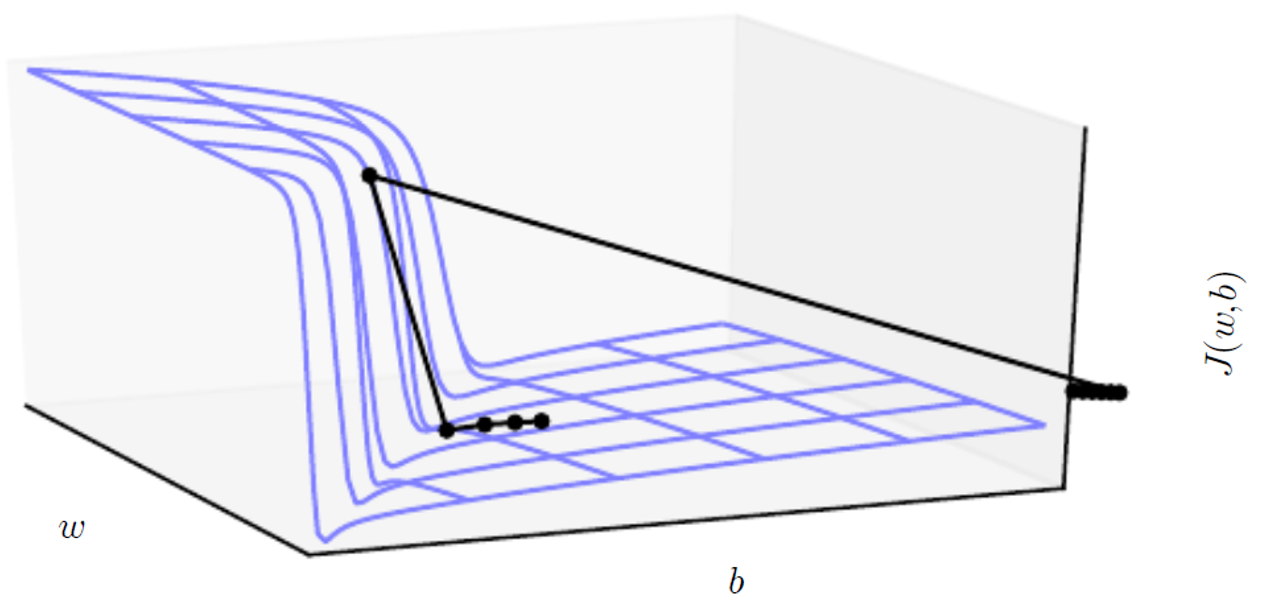
\includegraphics[width=0.9\linewidth]{images/cliff.png}
	\end{figure}


	\subsection{Long-Term Dependencies}
	Another difficulty that neural network optimization algorithms must overcome arises when the computational graph becomes extremely deep.
	Repeated application of the same parameters gives rise to especially pronounced diffculties.
	For example, suppose that a computational graph contains a path that consists of repeatedly multiplying by a matrix $\mW$.
	After $t$ steps, this is equivalent to multiplying by $\mW^t$.
	Suppose that $\mW$ has the following eigendecomposition:
	\begin{align*}
	\mW &= \mV \diag(\bol{\lambda})\mV^{-1}\\
	\mW^t &= \left(\mV \diag(\bol{\lambda})\mV^{-1}\right)^t = \mV \diag(\bol{\lambda})^t\mV^{-1}
 	\end{align*}


	In this simple case, it is straightforward to see that any eigenvalues $\lambda_i$ that are not near an absolute value of 1 will either explode if they are greater than 1 in magnitude or vanish if they are less than 1 in magnitude.\\

	The vanishing and exploding gradient problem refers to the fact that gradients through such a graph are also scaled according to $\diag(\bol{\lambda})^t$.
	\textbf{Vanishing gradients }make it difficult to know which direction the parameters should move to improve the cost function.
	\textbf{Exploding gradients} make learning unstable.

	\subsection{Algorithms with Adaptive Learning Rates \buch{Chapter 8.5}\buchSeite{298}}
		\subsubsection{Momentum}
		In all algorithms, we first calculate the gradient $g_t$ at time $t$ on a mini-batch of size $m$ with

		\[ g_{t} = \frac{1}{m} \nabla_{\Theta} \sum L(f(x^{(i)};\Theta),y^{(i)})    \]

		The final weight update is always given by

		\[ \Theta_{t} = \Theta_{t-1} + \Delta\Theta_{t} \]

		% The learning rate, if applicable, is denoted by $\theta$, and $\delta$ denotes a small constant (e.g. $ 10^{-6} $ or $ 10^{-8} $), which is required for numerical stability.

		\subsubsection{AdaGrad}
		The AdaGrad algorithm scales the learning rate of all model parameters by dividing them by the square root of the sum of all historical values of the gradient.

		\[ r_{t} = r_{t-1} + g_{t}\odot g_{t} \]
		\[ \Delta\Theta_{t} = - \frac{\eps}{\delta + \sqrt{r_{t}}} \odot g_{t} \]

		\subsubsection{RMSProp}
		The RMSProp algorithm is basically the same as AdaGrad, but the gradient is accumulated with an exponentially weighted moving average.

		\[ r_{t} = \rho r_{t-1} + (1- \rho) g_{t}\odot g_{t}\]
		\[ \Delta\Theta_{t} = - \frac{\eps}{\sqrt{\delta + r_{t}}} \odot g_{t} \]

		RMSProp combined with Nesterov momentum:

		\[ \tilde{\Theta_{t}} = \Theta_{t-1} + \alpha \Delta\Theta_{t-1} \]
		\[ g_{t} = \frac{1}{m} \nabla_{\tilde{\Theta_{t}}} \sum L(f(x^{(i)};\tilde{\Theta}),y^{(i)})    \]
		\[ r_{t} = \rho r_{t-1} + (1- \rho) g_{t}\odot g_{t}\]
		\[ \Delta\Theta_{t} = \alpha\Delta\Theta_{t-1} - \frac{\eps}{\sqrt{\delta + r_{t}}} \odot g_{t} \]

		\subsubsection{AdaDelta}
		AdaDelta is mentioned in the book, but not described. The idea is similar to RMSProp: the gradient is accumulated with an exponentially weighted moving average

		\[ r_{t} = \rho r_{t-1} + (1- \rho) g_{t}\odot g_{t}\]

		But now, we also accumulate the squared gradients using an exponentially weighted moving average

		\[ s_{t} = \rho s_{t-1} + (1 - \rho)\Delta\Theta_{t} \odot \Delta\Theta_{t} \]

		and use the accumulated squared gradient as the numerator in the gradient update

		\[ \Delta\Theta_{t} = - \frac{\sqrt{\delta + s_{t-1}}}{\sqrt{\delta + r_{t}}} \odot g_{t}\]

		Note that we first calculate the parameter update $ \Delta\Theta_{t} $ using the accumulated squared gradient of the last step $ s_{t-1} $, and then afterwards update the squared gradient $ s_{t} $. Thus, the accumulated squared gradient lags behind by one time step.\\
		AdaDelta has the advantage, that no learning rate $ \eps $ is required at all.

		\subsubsection{Adam}
		Adam (Adaptive Moments) goes one step further and accumulates the first- and second-order moments of the gradient to adapt the learning rate.

		\[ s_{t} = \rho_{1} s_{t-1} + (1 - \rho_{1})g_{t} \]
		\[ r_{t} = \rho_{2} r_{t-1} + (1 - \rho_{2})g_{t} \odot g_{t} \]

		The parameter update then uses the first-order moment of the gradient $ s_{t} $ instead of the gradient $ g_{t} $.

		\[ \Delta\Theta_{t} = -\eps\frac{\hat{s_{t}}}{\delta + \sqrt{\hat{r_{t}}}} \]

		Note that we use the bias-corrected versions $ \hat{s_{t}} = s_{t} / (1 - \rho_{1}^{t}) $ and $ \hat{r_{t}} = r_{t} / (1 - \rho_{2}^{t}) $, which are required due
		to the initialization at $ t = 0 $.

	\subsection{Batch Normalization}
	This is a method of adaptive re-parametrization, motivated by the difficulty of training very deep models.
	The gradient tells how to update each parameter, under the assumption that the other layers do not change.
	In practice, we update all of the layers simultaneously.
	When we make the update, unexpected results can happen because many functions composed together are changed simultaneously, using updates that were computed under the assumption that the other functions remain constant.\\

	Batch normalization provides a way of reparametrizing almost any deep network.
	The reparametrization significantly reduces the problem of coordinating updates across many layers.
	Batch normalization can be applied \textbf{to any input or hidden layer} in a network.\\

	Let $\mH$ be a minibatch of pre-activations of the layer to normalize arranged as a design matrix, with the pre-activations for each example appearing in a \textbf{row} of the matrix.
	To normalize $\mH$, we replace it with the expression
	\[ \mH'=\frac{\mH - \vmu}{\bol{\sigma}} \]

	The mean and the standard deviation per minibatch can be calculated during training:
	\begin{align*}
	\vmu &= \frac{1}{m}\sum_i\mH_{i,:}\\
	\bol{\sigma} &= \sqrt{\delta+\frac{1}{m}\sum_i (\mH-\vmu)_{i,:}^2}
	\end{align*}
	\textbf{Important:}
	We back-propagate through these operations for computing the mean and the standard deviation, and for applying them to normalize $\mH$. This means that the gradient will never propose an operation that acts simply to increase the standard deviation or mean of any pre-activation. The normalization operations remove the effect of such an action and zero out its component in the gradient. Hence the mean of the pre-activation stays at zero and the standard deviation at one over a minibatch, which solves many problems related to exploding and vanishing gradients.


	\subsection{Parameter Initialization Strategies \buch{Chapter 8.4}\buchSeite{292}}
	A few things to know about what the initialization does affect:
	\begin{itemize}
		\item Most algorithms are strongly affected by the choice of initialization
		\item The initial point can determine whether the algorithm converges at all
		\item When learning does converge, the initial point can determine how quickly learning converges and whether it converges to a point with high or low cost
		\item Also, points of comparable cost can have wildly varying generalization error, and the initial point can affect the generalization as well
	\end{itemize}

	The initialization strategies used today are simple and heuristic. Hence we don't know much about
	how the initial point affects generalization. So there's little to no guidance how to select the initial point of the parameters.\\
	The only property known with complete certainty is that the initial parameters need to “break symmetry” between different units. If two hidden units with the same activation function are connected to the same inputs leads during training to constantly update both of these units in the same way.\\
	The goal of having each unit compute a different function motivates	random initialization of the parameters. Typically we set the biases for each unit to a heuristically chosen constant (0 is popular (0.1 for ReLu)).We almost always initialize all the weights in the model to values drawn randomly from a Gaussian or uniform distribution.\\
	\textbf{Larger initial }weights will yield a stronger symmetry breaking effect, helping to avoid redundant units. They also help to avoid losing signal during forward- or back-propagation through the linear component of each layer. If the initial weights get \textbf{too large} it can result in exploding values during forward- or back-propagation (Maybe clipping gradient can be used to avoid those effects).\\

	A heuristic is to initialize the weights of a fully connected layer with m inputs and n outputs by sampling each weight from the uniform distribution shown below. Which leads to:
	\[  U(-\frac{\sqrt{3}}{\sqrt{m}}, \frac{\sqrt{3}}{\sqrt{m}}) \]

	\begin{figure}[H]
		\centering
		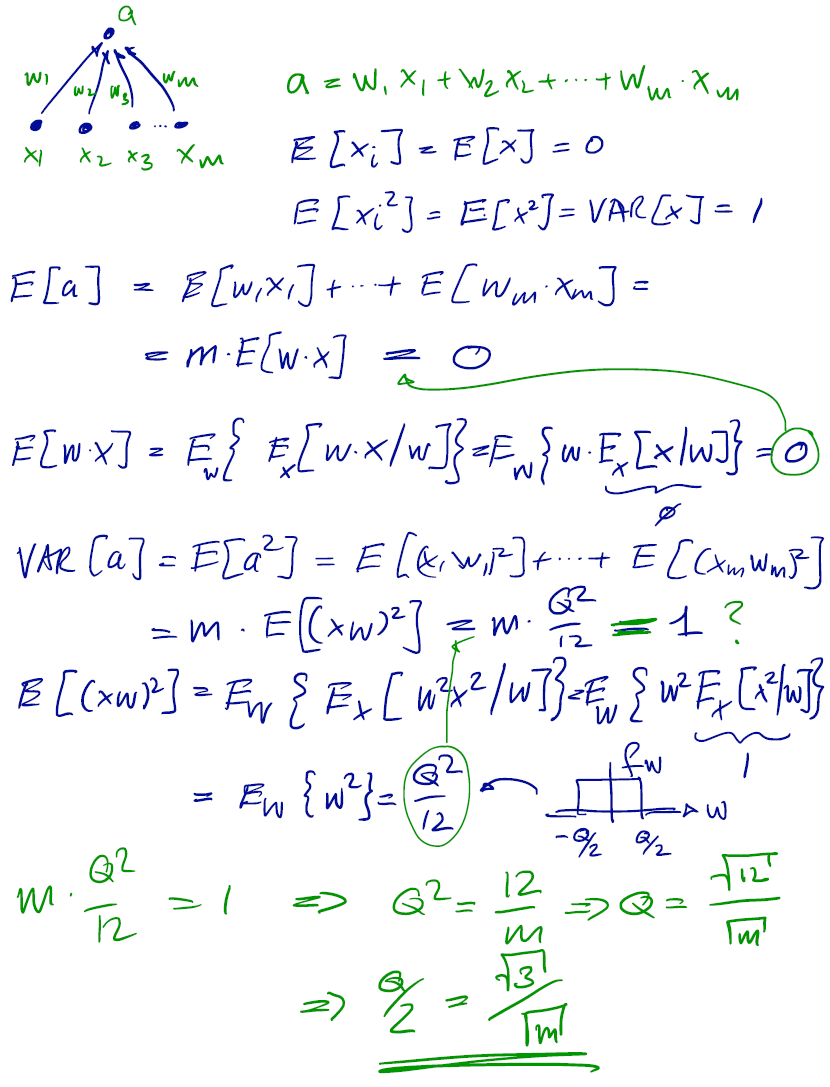
\includegraphics[width=0.9\linewidth]{images/InitStrat.png}
	\end{figure}

	Normalized initialization: This heuristic is designed to compromise between the goal of initializing all layers to have the same pre-activation variance and the goal of initializing all layers to have the same gradient variance. The formula is derived using the assumption that the network consists only of a chain of matrix multiplications, with no nonlinearities.

	\[ W_{i,j} \sim\ U ( -\frac{\sqrt{6}}{\sqrt{m + n}}, \frac{\sqrt{6}}{\sqrt{m + n}} )  \]

	This strategy is often called the \textbf{Xavier Initialization}.\\
	There are some more strategies which are often applied in neural networks which we will not go into further details.



	\newpage
\end{multicols}
